\section*{Motivation}

\begin{frame}{Anwendungsfall E-Commerce I}
    \begin{itemize}
        \item Ziel: Backend für internationales E-Commerce-System
        \item MVP: Bestellungen, Bezahlung und Versand
        \item Zukünftig viele Nutzer und hoher Traffic erwartet
        \item Geringes Kapital für Infrastruktur
        \item Rechtliche Regularien teilweise unklar, weil international
        \item Hohe Sicherheitsanforderungen
        \item Agiles Team von acht fähigen Entwicklern
        \item Geldgeber wollen erste Auslieferung in zwei Wochen
    \end{itemize}
\end{frame}

\begin{frame}{Anwendungsfall E-Commerce II}
    \begin{figure}[!h]
        \centering
        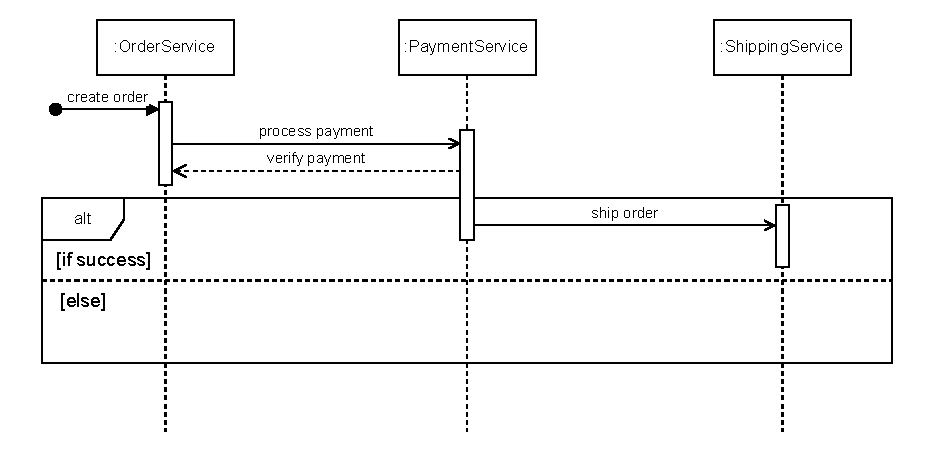
\includegraphics[scale=0.65]{imglib/einleitung/ecommerce.drawio}
        \caption{Sequenzdiagram zum Aufgeben einer Bestellung}
        \label{fig:ecommerce}
    \end{figure}
\end{frame}

\begin{frame}{Grundlagen und Anforderungen}
    \begin{itemize}
        \item Architectura lateinisch für: \textit{Wissenschaft der Baukunst}
        \item Software-Architektur: Grundlegende Struktur und Beziehungen von Teilen einer Software \cite{eaprinciples}
        \item Enterprise-Architektur (EA): Grundlegende Struktur und Beziehungen von Komponenten eines Systems
        \item EA beschreibt Prozess und Ergebnis (vgl. Bedeutung latein. \textit{architectura})
        \item Ziel: Ausrichtung von Business und IT
        \item Umsetzung durch EA-Muster: Spezifische Strategien zur Ausrichtung
    \end{itemize}
\end{frame}
